\chapter{Triển khai}

% Phụ trách: .............

Chương này trình bày quá trình triển khai hệ thống quản lý bãi giữ xe
dựa trên thiết kế đã được xây dựng ở Chương~4. Nội dung bao gồm môi
trường phát triển, cấu trúc mã nguồn và cách hiện thực các chức năng
chính của hệ thống bằng ngôn ngữ C\#, Windows Forms và SQL Server.

% ==================================================
\section{Môi trường và công nghệ}
% ==================================================

Hệ thống được xây dựng trên nền tảng Microsoft .NET Framework với
ngôn ngữ lập trình C\# và cơ sở dữ liệu SQL Server. Các công cụ sử
dụng trong quá trình phát triển được trình bày trong
Bảng~\ref{tab:congcu}.

\begin{table}[htbp]
    \centering
    \begin{tabular}{lll}
        \toprule
        \textbf{Công cụ} &
        \textbf{Phiên bản} &
        \textbf{Mục đích sử dụng} \\
        \midrule
        Visual Studio & 2022 & Phát triển ứng dụng C\# \\
        .NET Framework & 4.8 & Nền tảng chạy chương trình \\
        SQL Server & 2022 & Hệ quản trị cơ sở dữ liệu \\
        SSMS & 19.x & Quản trị cơ sở dữ liệu \\
        Git & 2.x & Quản lý mã nguồn \\
        GitHub & Online & Lưu trữ và chia sẻ dự án \\
        \bottomrule
    \end{tabular}
    \caption{Các công cụ sử dụng trong dự án}
    \label{tab:congcu}
\end{table}

Hệ thống được kiểm thử trên máy tính sử dụng hệ điều hành Windows 10
và Windows 11. Việc truy cập cơ sở dữ liệu được thực hiện thông qua
ADO.NET với cơ chế truy vấn tham số hóa nhằm bảo đảm an toàn dữ liệu.

% ==================================================
\section{Cấu trúc project}
% ==================================================

Dự án được tổ chức theo mô hình ba lớp gồm BLL, DAL, Model và Presenters nhằm
tách biệt các chức năng của hệ thống.

\begin{verbatim}
ParkingManagement
|
|-- DAL
|   |-- BangGiaDAL
|   |-- ChoTrongDAL
|   |-- Database
|   |-- KhachHangDAL
|   |-- LoaiXeDAL
|   |-- LuotGuiDAL
|   |-- NhatKyDAL
|   |-- TaiKhoanDAL
|   |-- TheXeDAL
|   |-- ThongKeDAL
|   |-- TraCuuDAL
|   |-- VeThangDAL
|
|-- BLL
|   |-- BangGiaBLL
|   |-- BaoCaoBLL
|   |-- BaoMat
|   |-- ChoTrongBLL
|   |-- KhachHangBLL
|   |-- LoaiXeBLL
|   |-- LuotGuiBLL
|   |-- NhatKyBLL
|   |-- PhienLamViec
|   |-- TaiKhoanBLL
|   |-- TheXeBLL
|   |-- TinhPhiBLL
|   |-- TraCuuBLL
|   |-- VeThangBLL
|
|-- Model
|   |-- BangGiaDTO.cs
|   |-- BienNhanDTO.cs
|   |-- ChoTrongDTO.cs
|   |-- DoanhThuDTO.cs
|   |-- GioCaoDiemDTO.cs
|   |-- GoiYVeThangDTO.cs
|   |-- KetQua.cs
|   |-- KhachHangDTO.cs
|   |-- LoaiXeDTO.cs
|   |-- LuotGuiDTO.cs
|   |-- NhatKyDTO.cs
|   |-- OGuiDTO.cs
|   |-- TaiKhoanDTO.cs
|   |-- ThanhToanDTO.cs
|   |-- TheXeDTO.cs
|   |-- VeThangDTO.cs
|
|-- Presenters
|   |-- BangGiaPresenter.cs
|   |-- BaoCaoPresenter.cs
|   |-- DangNhapPresenter.cs
|   |-- DoiMatKhauPresenter.cs
|   |-- KhachHangPresenter.cs
|   |-- LoaiXePresenter.cs
|   |-- NhatKyPresenter.cs
|   |-- TheXePresenter.cs
|   |-- TraCuuPresenter.cs
|   |-- VanHanhPresenter.cs
|   |-- VeThangPresenter.cs
|
|-- View
|   |-- FrmDangNhap
|   |-- Frmdoimatkhau
|   |-- IBangGiaView
|   |-- IBaoCaoView
|   |-- ucBangGia
|   |-- ucBaoCao
|   |-- ucVeThang
|   |-- ...
|
|
|
|-- Utils
\end{verbatim}

Trong đó:

\begin{itemize}
    \item \textbf{View:} Chứa các Form giao diện người dùng.

    \item \textbf{BLL:} Xử lý các nghiệp vụ của hệ thống.

    \item \textbf{DAL:} Thực hiện truy cập cơ sở dữ liệu.

    \item \textbf{DTO:} Chứa các lớp biểu diễn dữ liệu.

    \item \textbf{Utils:} Chứa các lớp hỗ trợ dùng chung.
\end{itemize}

% ==================================================
\section{Module ghi nhận xe vào}
% ==================================================

Khi xe vào bãi, nhân viên nhập biển số xe, chọn loại xe và thẻ xe.
Hệ thống kiểm tra trạng thái của thẻ trước khi tạo lượt gửi mới.

Đối tượng lượt gửi được khởi tạo như sau:

\begin{lstlisting}
LuotGui luot = new LuotGui()
{
    TheXeID = theXeId,
    LoaiXeID = loaiXeId,
    BienSoXe = txtBienSo.Text.Trim(),
    GioVao = DateTime.Now
};
\end{lstlisting}

Sau khi lưu thành công, hệ thống cập nhật trạng thái thẻ xe sang
đang sử dụng:

\begin{lstlisting}
theXeBLL.CapNhatTrangThai(
    theXeId,
    true
);
\end{lstlisting}

Việc ghi nhận giờ vào bằng \texttt{DateTime.Now} giúp bảo đảm tính
chính xác và tránh sai sót do nhập tay.

% ==================================================
\section{Module tính phí}
% ==================================================

Tính phí là nghiệp vụ quan trọng của hệ thống. Số tiền gửi xe được
xác định dựa trên thời gian gửi và đơn giá của từng loại xe.

Đề tài sử dụng delegate \texttt{Func} để biểu diễn công thức tính
phí. Cách tiếp cận này giúp dễ dàng thay đổi chính sách giá mà
không ảnh hưởng tới các phần khác của hệ thống.

\begin{lstlisting}
// Vi du: cong thuc tinh phi dung Func
Func<DateTime, DateTime, decimal, decimal> tinhPhi =
    (vao, ra, giaMoiGio) =>
    {
        var gio = Math.Ceiling(
            (ra - vao).TotalHours
        );

        return (decimal)gio * giaMoiGio;
    };
\end{lstlisting}

Khi xe gửi dưới một giờ, hệ thống vẫn tính tối thiểu một giờ theo
quy định của bãi xe.

\begin{lstlisting}
if (gio < 1)
{
    gio = 1;
}
\end{lstlisting}

Đối với xe có vé tháng còn hiệu lực, hệ thống trả về giá trị bằng 0.

\begin{lstlisting}
if (veThangConHan)
{
    return 0;
}
\end{lstlisting}

% ==================================================
\section{Module xe ra và transaction thanh toán}
% ==================================================

Khi xe ra, hệ thống phải thực hiện đồng thời nhiều thao tác:

\begin{enumerate}
    \item Ghi nhận giờ ra.
    \item Tính phí gửi xe.
    \item Ghi giao dịch thanh toán.
    \item Giải phóng thẻ xe.
\end{enumerate}

Để bảo đảm tính toàn vẹn dữ liệu, các thao tác trên được thực hiện
trong một transaction.

\begin{lstlisting}
using (SqlConnection conn =
       new SqlConnection(connectionString))
{
    conn.Open();

    SqlTransaction tran = conn.BeginTransaction();

    try
    {
        // Cap nhat luot gui
        // Ghi thanh toan
        // Giai phong the xe

        tran.Commit();
    }
    catch
    {
        tran.Rollback();
        throw;
    }
}
\end{lstlisting}

Nhờ cơ chế transaction, hệ thống tránh được các trường hợp chỉ
cập nhật một phần dữ liệu khi xảy ra lỗi.

% ==================================================
\section{Module quản lý vé tháng}
% ==================================================

Chức năng quản lý vé tháng cho phép đăng ký mới, gia hạn và kiểm
tra tình trạng vé của khách hàng.

Khi đăng ký vé tháng, hệ thống tự động tính ngày hết hạn dựa trên
thời gian đăng ký.

\begin{lstlisting}
VeThang ve = new VeThang()
{
    KhachHangID = khachHangID,
    TheXeID = theXeID,
    NgayBatDau = DateTime.Today,
    NgayHetHan = DateTime.Today.AddMonths(1)
};
\end{lstlisting}

Khi gia hạn, hệ thống cập nhật lại ngày hết hạn tương ứng.

\begin{lstlisting}
ve.NgayHetHan = ve.NgayHetHan.AddMonths(1);
\end{lstlisting}

Trong quá trình xe ra, hệ thống kiểm tra ngày hết hạn của vé tháng
trước khi tính phí gửi xe.

% ==================================================
\section{Module tra cứu lịch sử}
% ==================================================

Chức năng tra cứu cho phép tìm kiếm các lượt gửi theo biển số,
mã thẻ hoặc khoảng thời gian.

Ví dụ truy vấn theo biển số:

\begin{lstlisting}[language=SQL]
SELECT *
FROM LuotGui
WHERE BienSoXe LIKE @BienSoXe;
\end{lstlisting}

Ví dụ tra cứu theo khoảng thời gian:

\begin{lstlisting}[language=SQL]
SELECT *
FROM LuotGui
WHERE GioVao BETWEEN @TuNgay AND @DenNgay;
\end{lstlisting}

Kết quả được hiển thị trên điều khiển \texttt{DataGridView},
hỗ trợ người dùng dễ dàng kiểm tra lịch sử gửi xe.

% ==================================================
\section{Module in vé và biên nhận}
% ==================================================

Hệ thống sử dụng lớp \texttt{PrintDocument} của .NET Framework
để thực hiện chức năng in.

\begin{lstlisting}
PrintDocument pd = new PrintDocument();

pd.PrintPage += PrintPageHandler;

pd.Print();
\end{lstlisting}

Thông tin in trên vé gồm:

\begin{itemize}
    \item Mã thẻ xe.
    \item Biển số xe.
    \item Loại xe.
    \item Thời gian vào bãi.
\end{itemize}

Biên nhận thanh toán khi xe ra bổ sung thêm:

\begin{itemize}
    \item Thời gian ra bãi.
    \item Thời gian gửi.
    \item Số tiền thanh toán.
\end{itemize}

% ==================================================
\section{Giao diện chương trình}
% ==================================================

Các giao diện của hệ thống quản lý bãi giữ xe được xây dựng bằng Windows Forms với tiêu chí trực quan, đơn giản và dễ sử dụng cho nhân viên cũng như người quản lý.

\subsection{Giao diện đăng nhập và vận hành (Xe vào)}
Giao diện đăng nhập cho phép phân quyền người dùng, kết hợp màn hình vận hành hỗ trợ ghi nhận xe vào bãi nhanh chóng.

\begin{figure}
    \centering
    \begin{minipage}{0.48\textwidth}
        \centering
        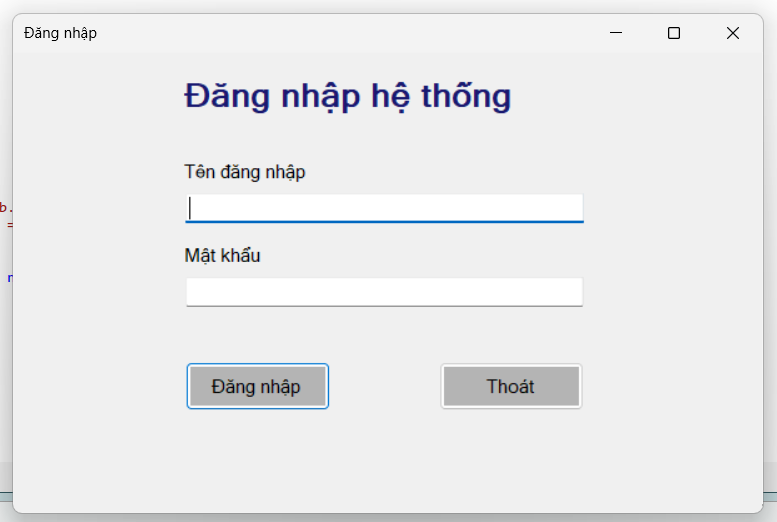
\includegraphics[width=\linewidth]{images/dang-nhap.png}
        \caption{Giao diện đăng nhập}
    \label{fig:dang-nhap}
    \end{minipage}
    \hfill
    \begin{minipage}{0.48\textwidth}
        \centering
        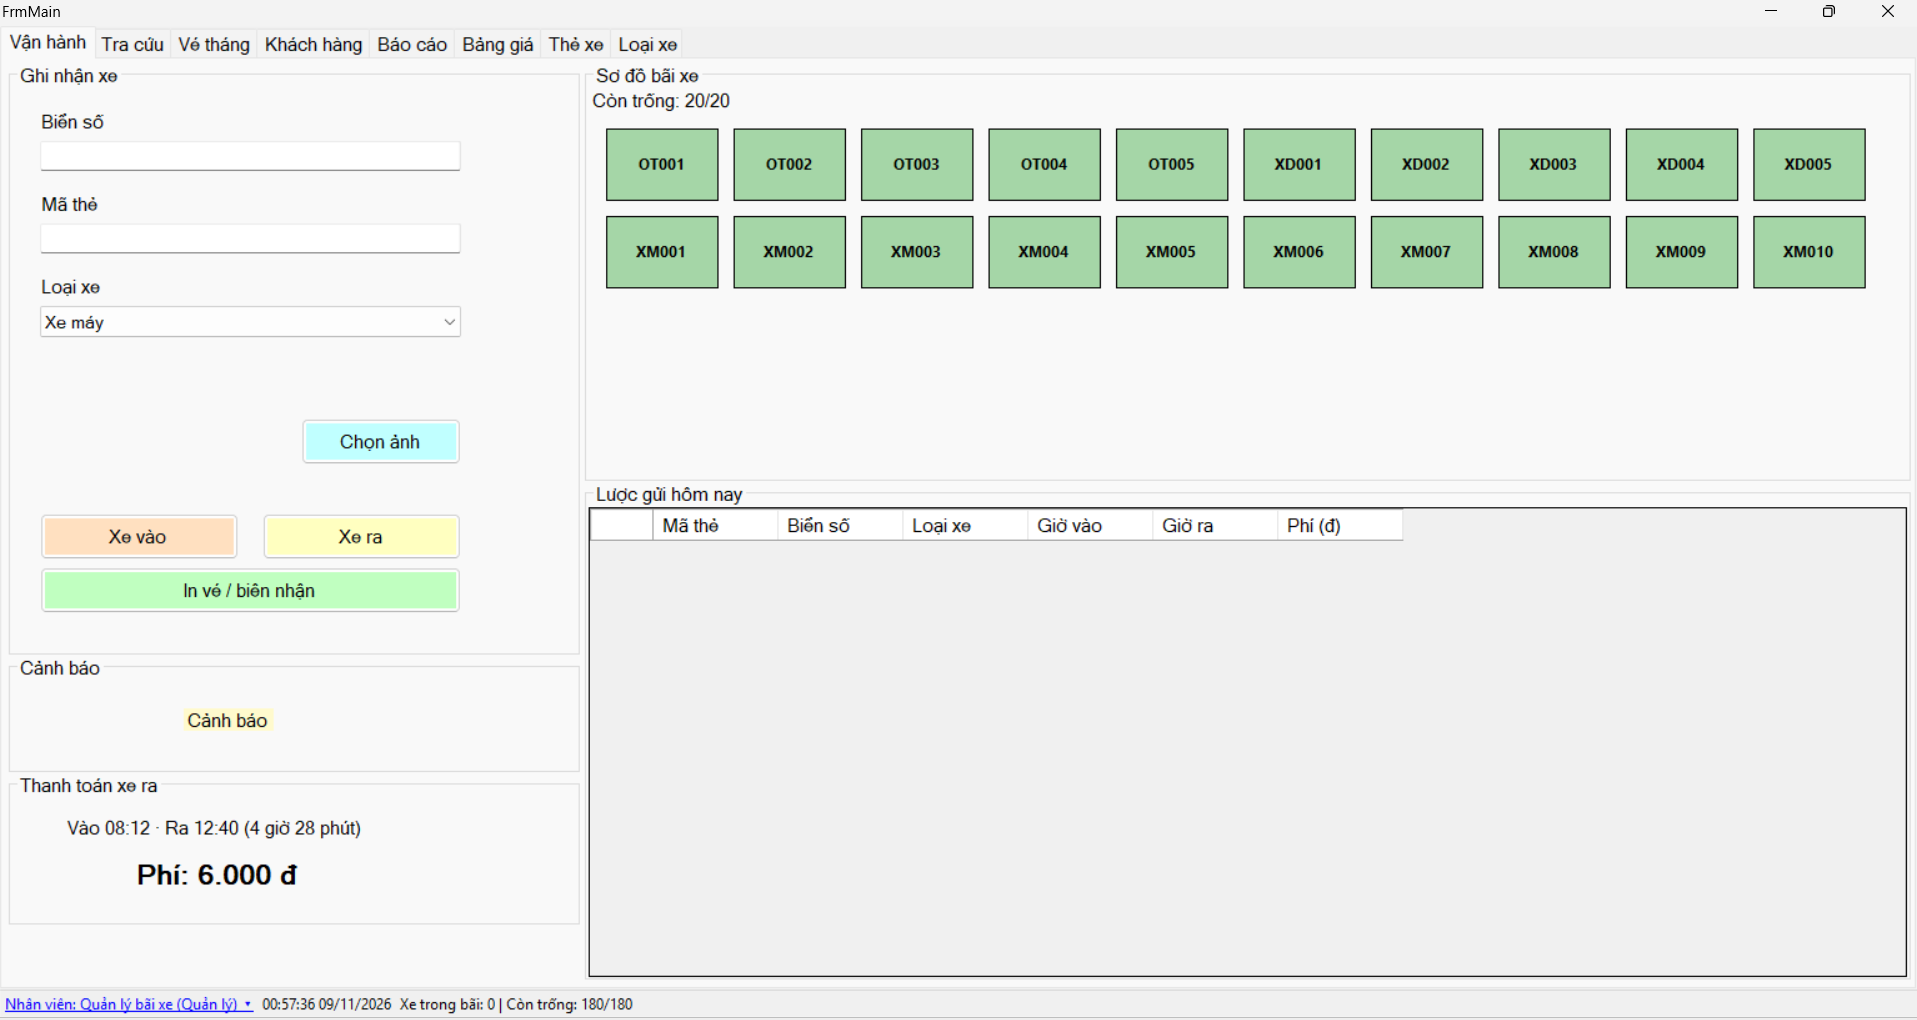
\includegraphics[width=\linewidth]{images/gd-van-hanh.png}
        \caption{Giao diện ghi nhận xe vào}
        \label{fig:xe-vao}
    \end{minipage}
\end{figure}

\subsection{Giao diện tra cứu và quản lý vé tháng}
Màn hình hỗ trợ tra cứu lượt gửi xe, tính phí thanh toán và quản lý thông tin đăng ký vé tháng cho khách hàng.

\begin{figure}
    \centering
    \begin{minipage}{0.48\textwidth}
        \centering
        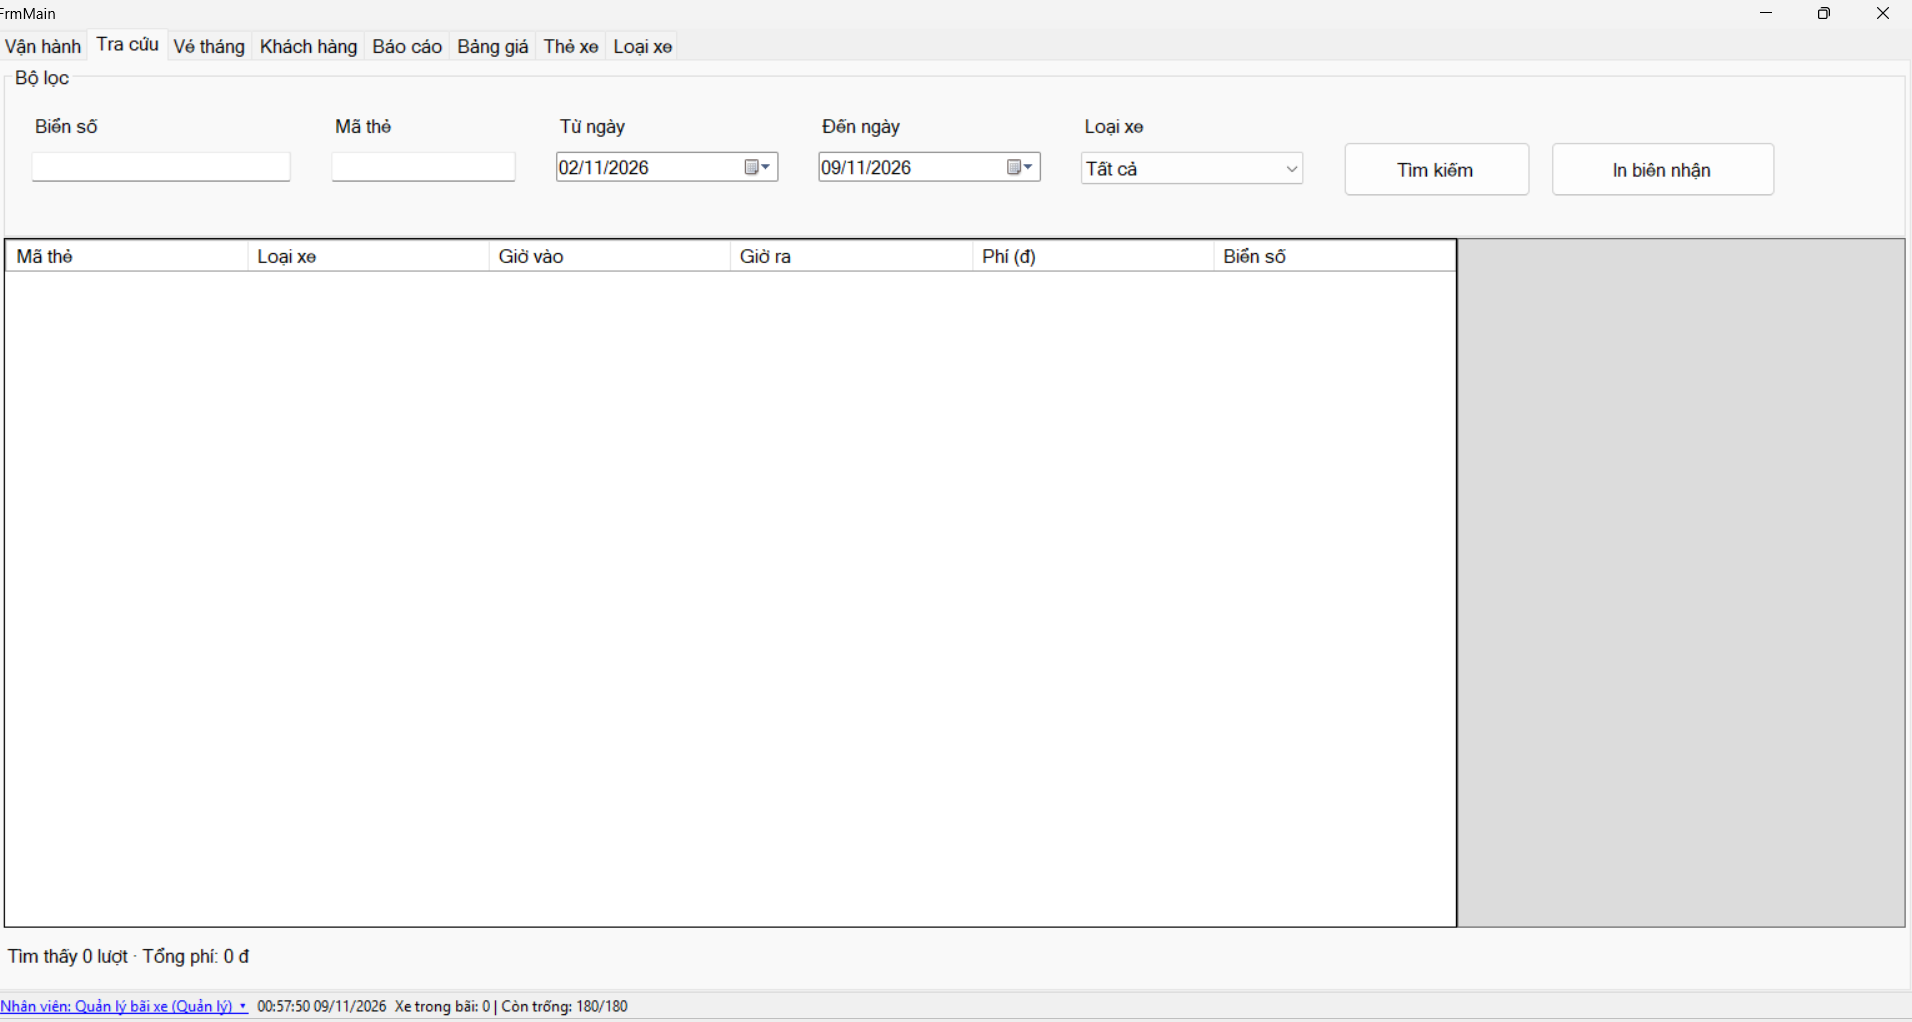
\includegraphics[width=\linewidth]{images/gd-tra-cuu.png}
        \caption{Giao diện tra cứu xe ra}
        \label{fig:tra-cuu}
    \end{minipage}
    \hfill
    \begin{minipage}{0.48\textwidth}
        \centering
        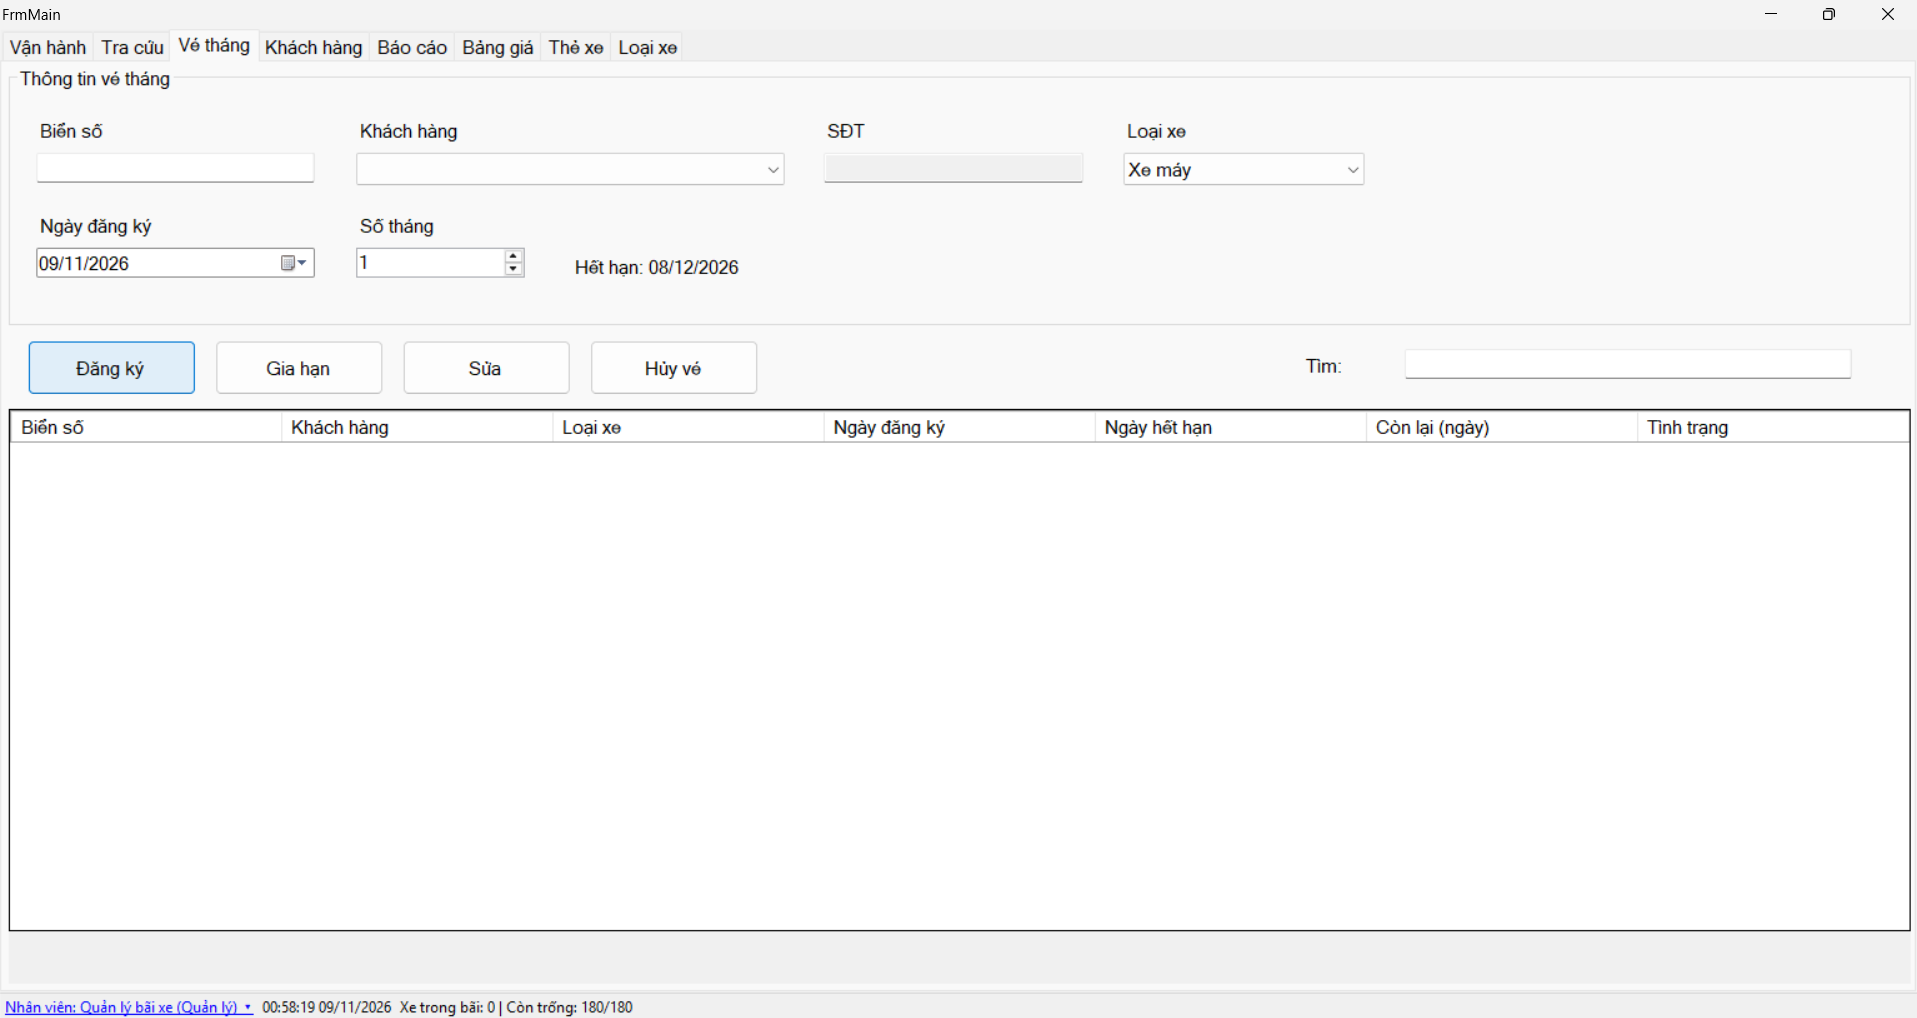
\includegraphics[width=\linewidth]{images/gd-ve-thang.png}
        \caption{Giao diện quản lý vé tháng}
        \label{fig:ve-thang}
    \end{minipage}
\end{figure}

\subsection{Giao diện quản lý khách hàng và thẻ xe}
Màn hình lưu trữ thông tin khách hàng định kỳ và quản lý trạng thái các thẻ xe trong hệ thống.

\begin{figure}
    \centering
    \begin{minipage}{0.48\textwidth}
        \centering
        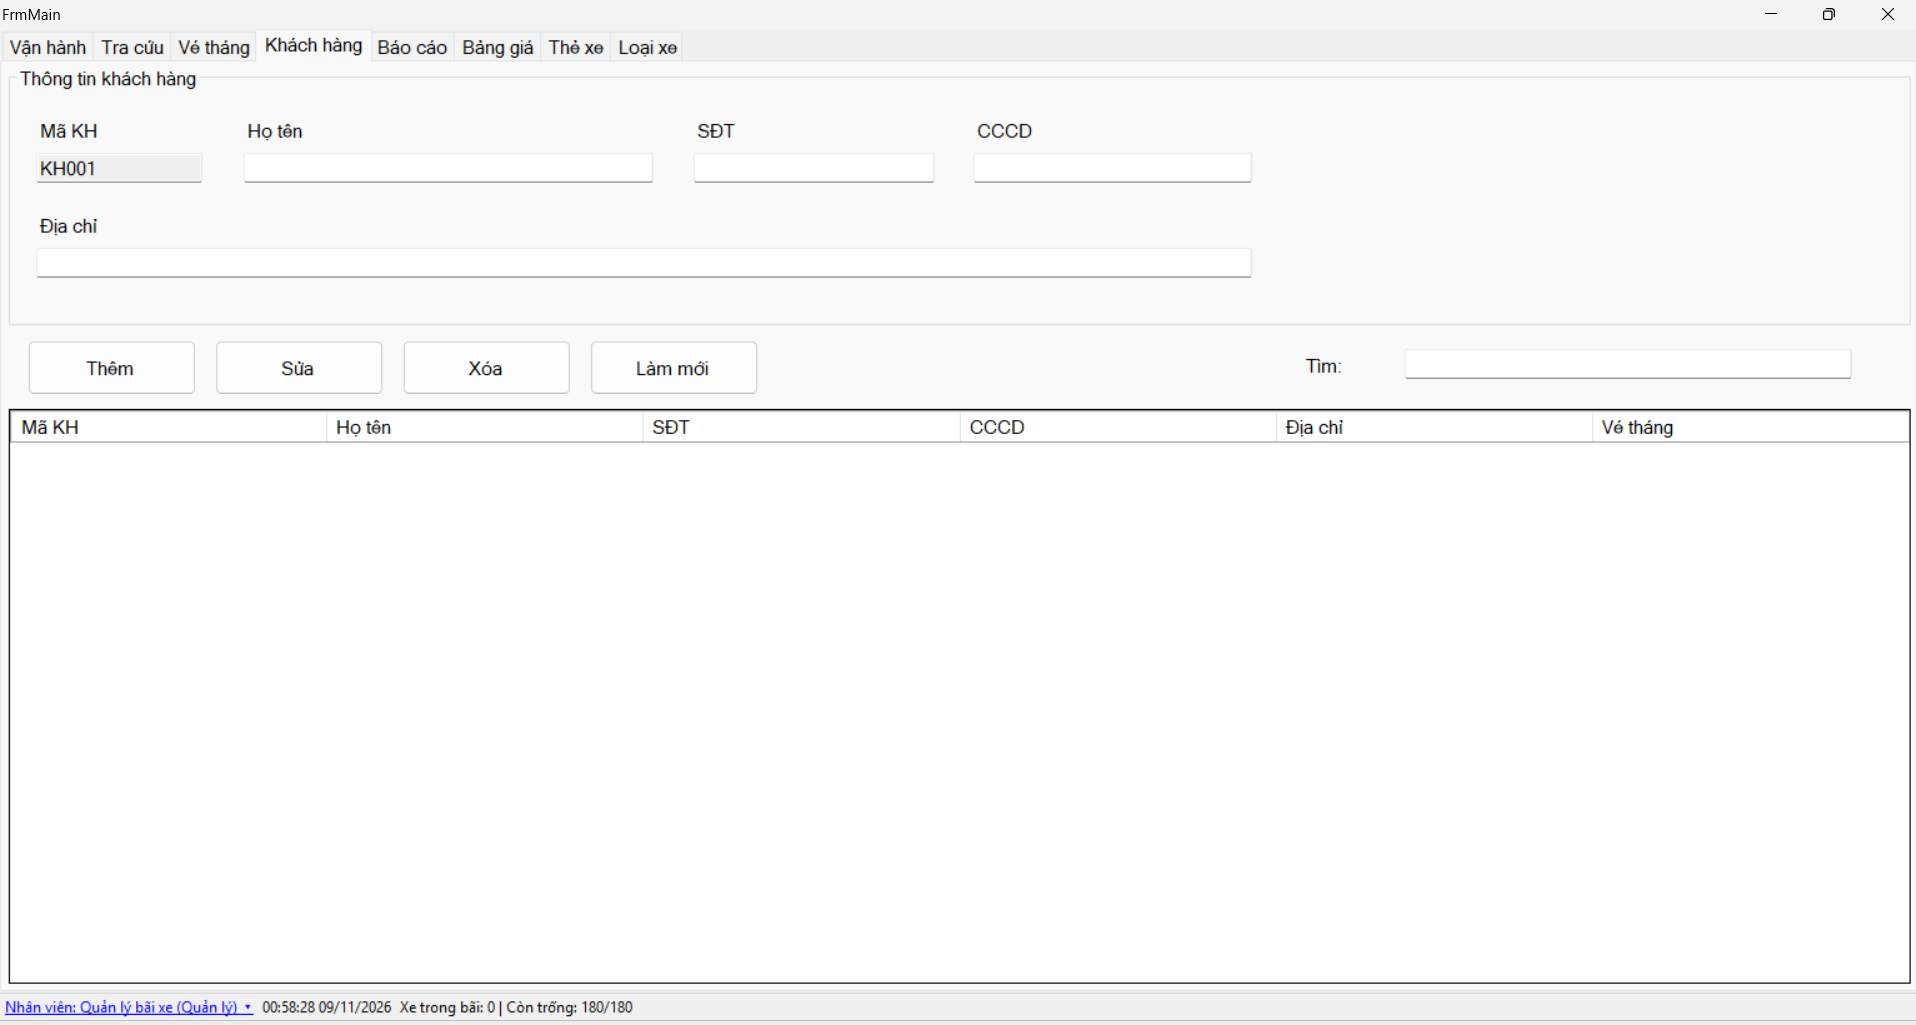
\includegraphics[width=\linewidth]{images/gd-khach-hang.png}
        \caption{Giao diện khách hàng}
        \label{fig:khach-hang}
    \end{minipage}
    \hfill
    \begin{minipage}{0.48\textwidth}
        \centering
        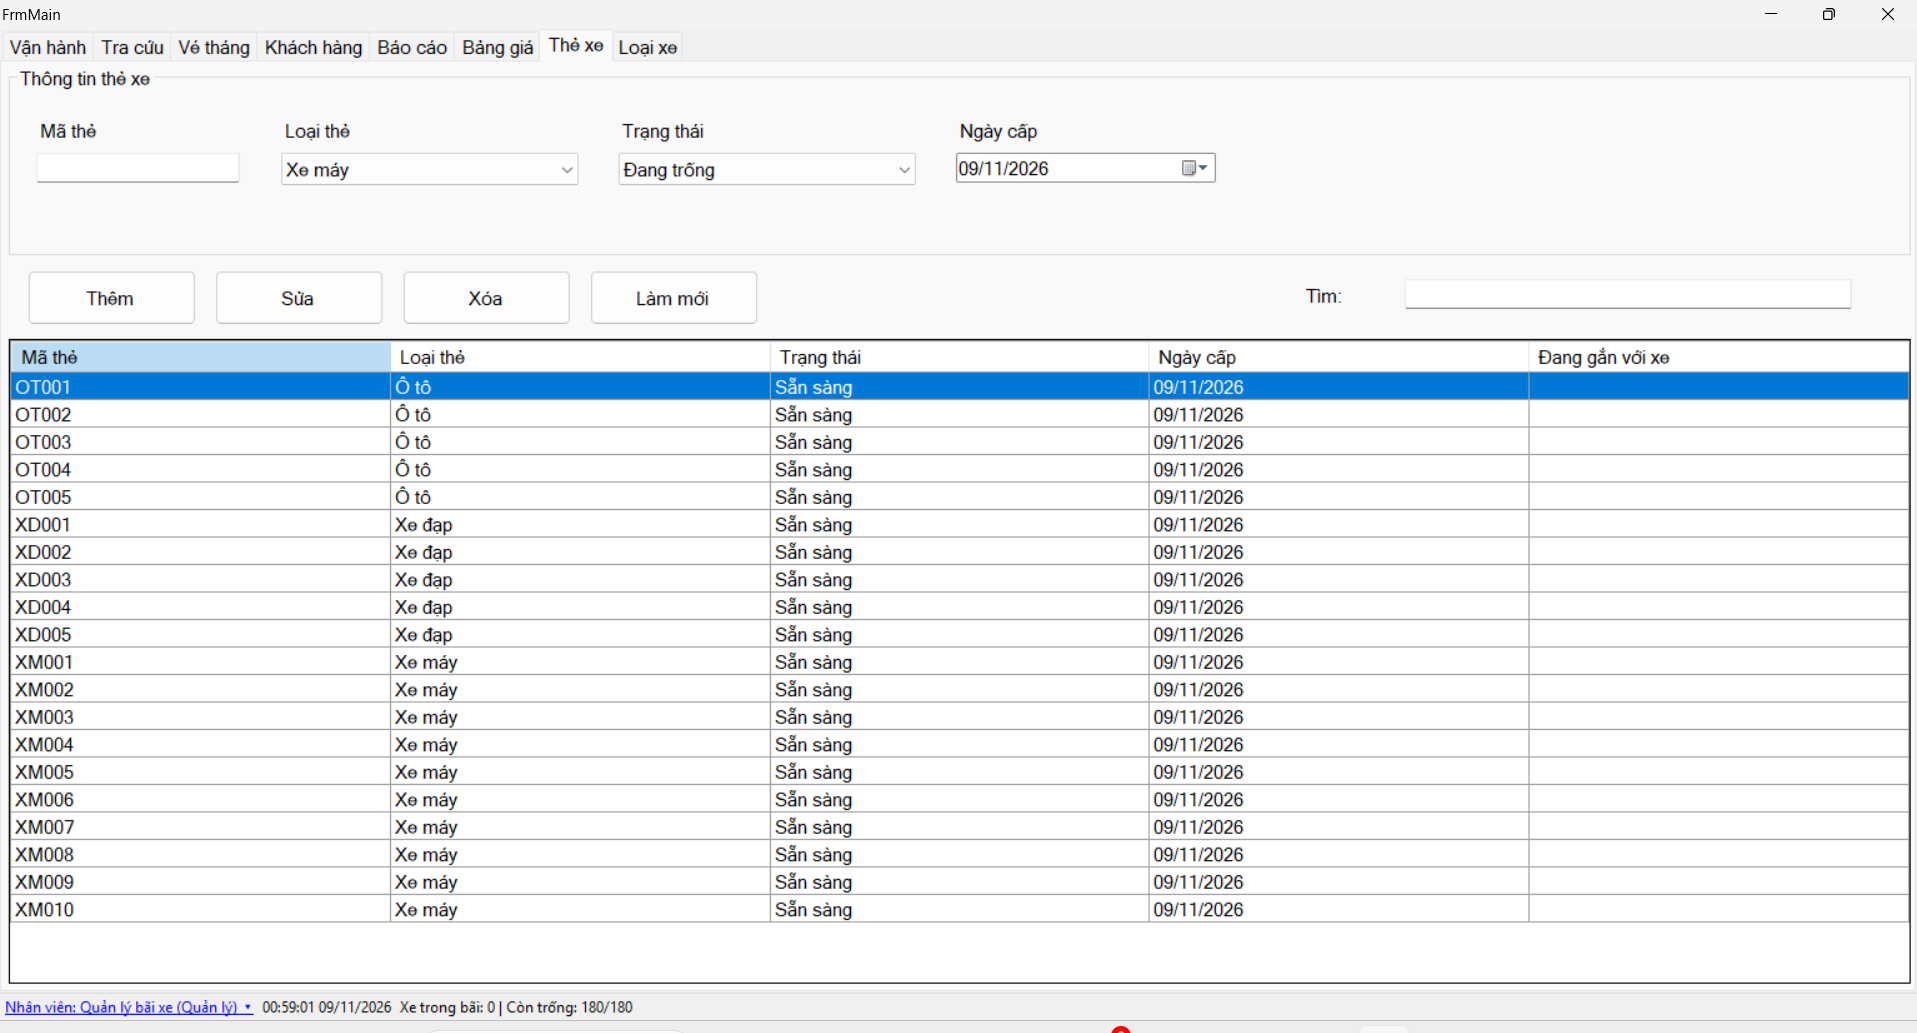
\includegraphics[width=\linewidth]{images/gd-the-xe.png}
        \caption{Giao diện thẻ xe}
        \label{fig:the-xe}
    \end{minipage}
\end{figure}

\subsection{Giao diện quản lý loại xe và bảng giá}
Màn hình cấu hình loại phương tiện và thiết lập các mức giá gửi xe theo giờ, qua đêm hoặc vé tháng.

\begin{figure}
    \centering
    \begin{minipage}{0.48\textwidth}
        \centering
        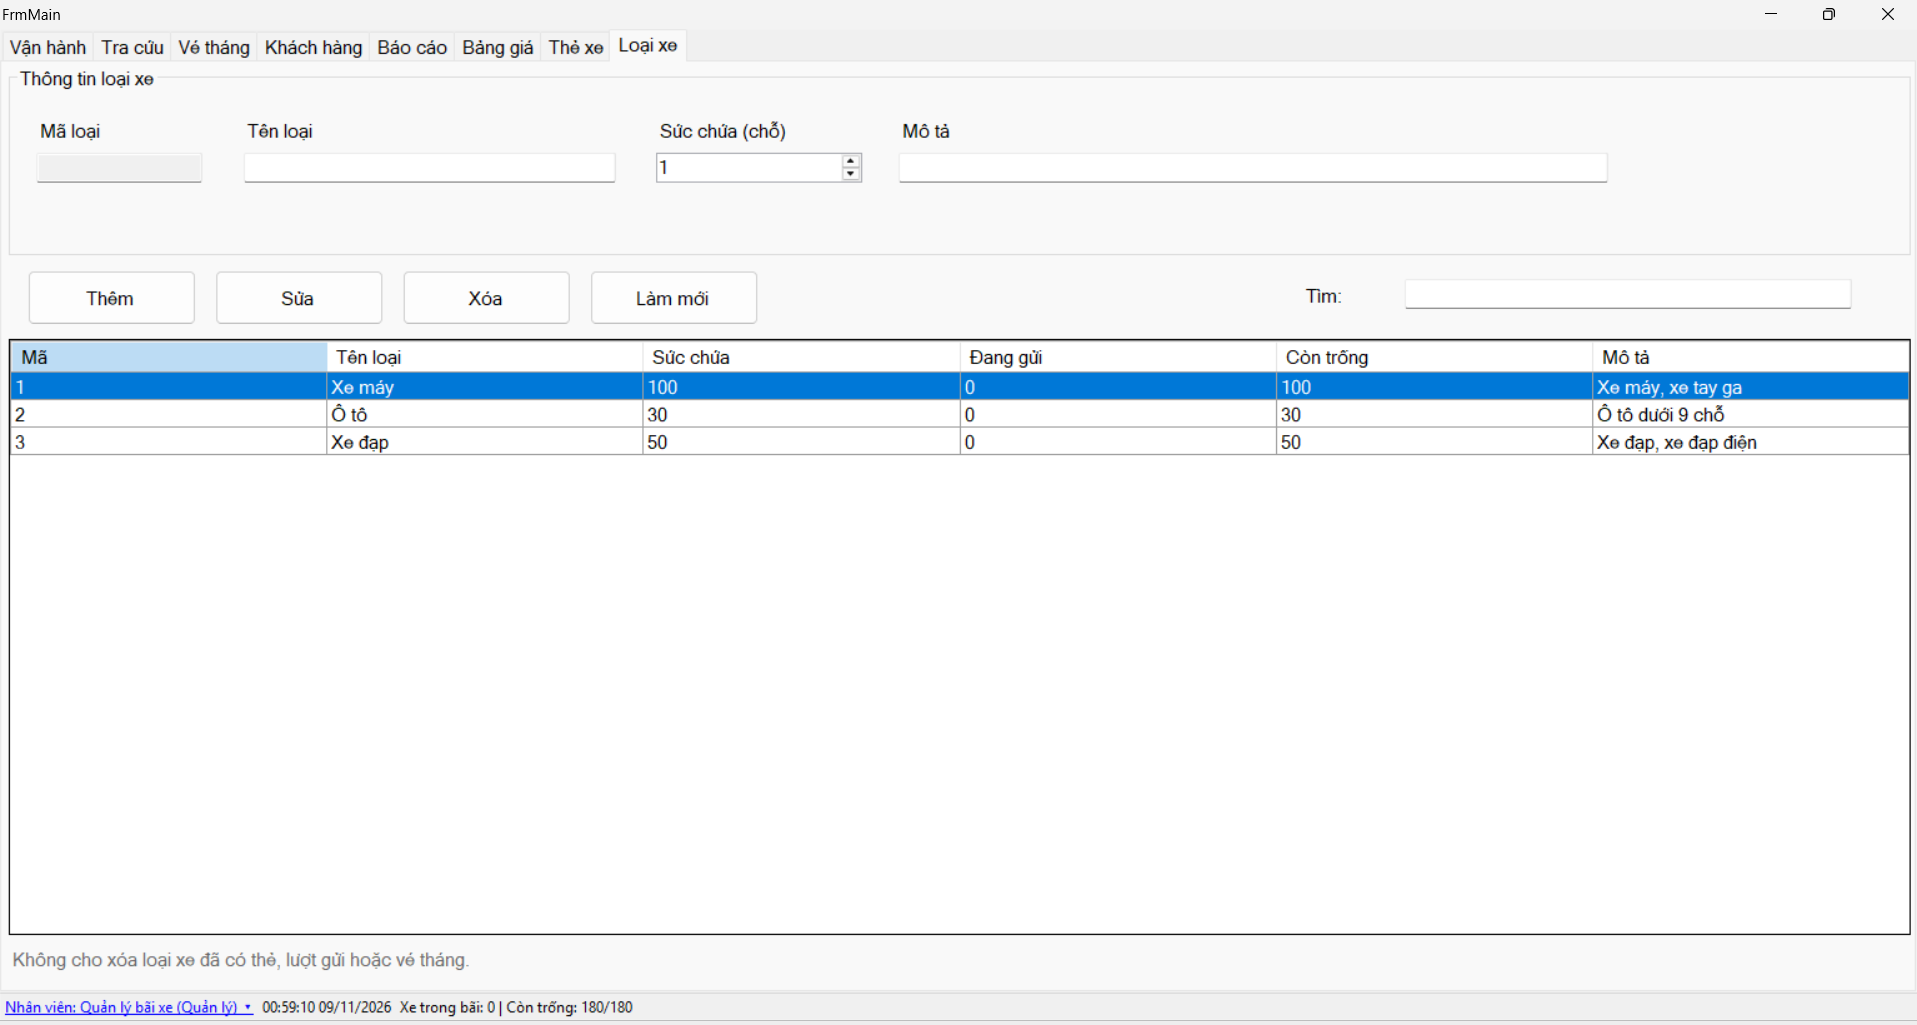
\includegraphics[width=\linewidth]{images/gd-loai-xe.png}
        \caption{Giao diện loại xe}
        \label{fig:loai-xe}
    \end{minipage}
    \hfill
    \begin{minipage}{0.48\textwidth}
        \centering
        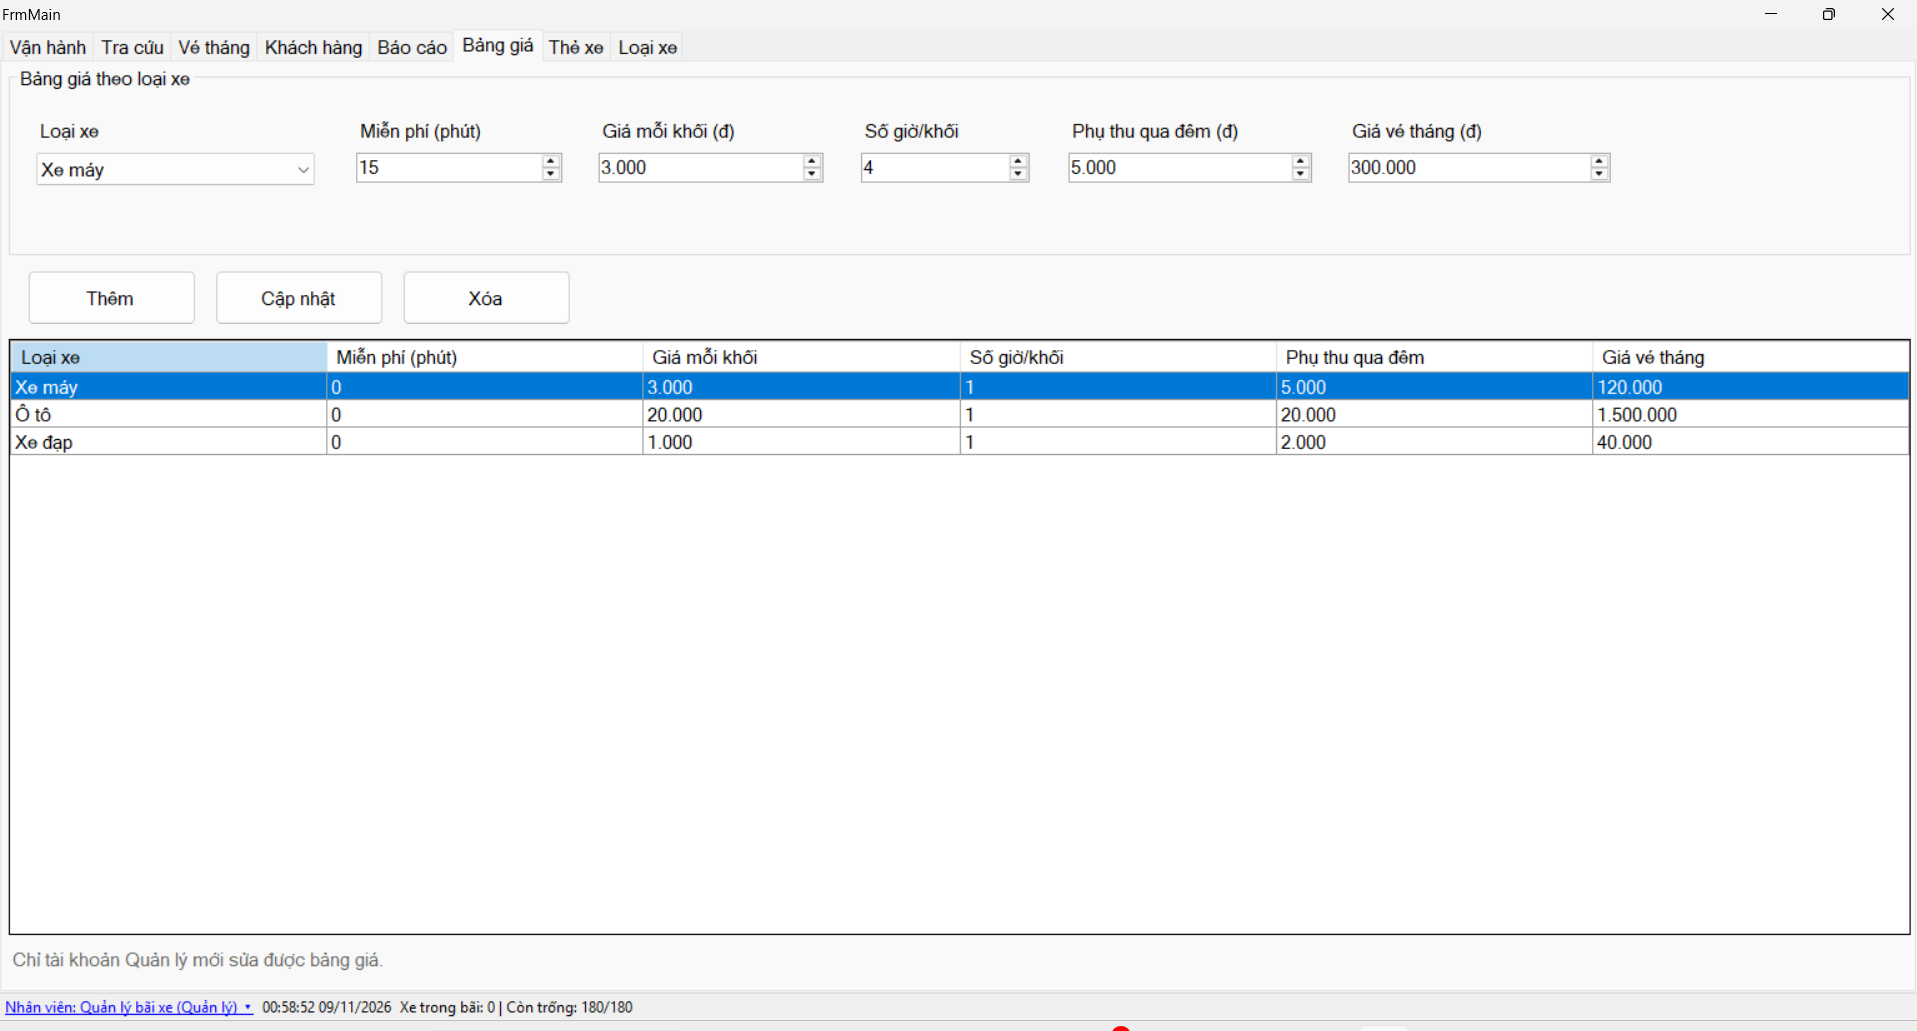
\includegraphics[width=\linewidth]{images/gd-bang-gia.png}
        \caption{Giao diện bảng giá}
        \label{fig:bang-gia}
    \end{minipage}
\end{figure}

\subsection{Giao diện thống kê báo cáo doanh thu}
Màn hình tổng hợp số liệu doanh thu chi tiết theo ngày, tháng để phục vụ công tác quản lý tài chính.

\begin{figure}
    \centering
    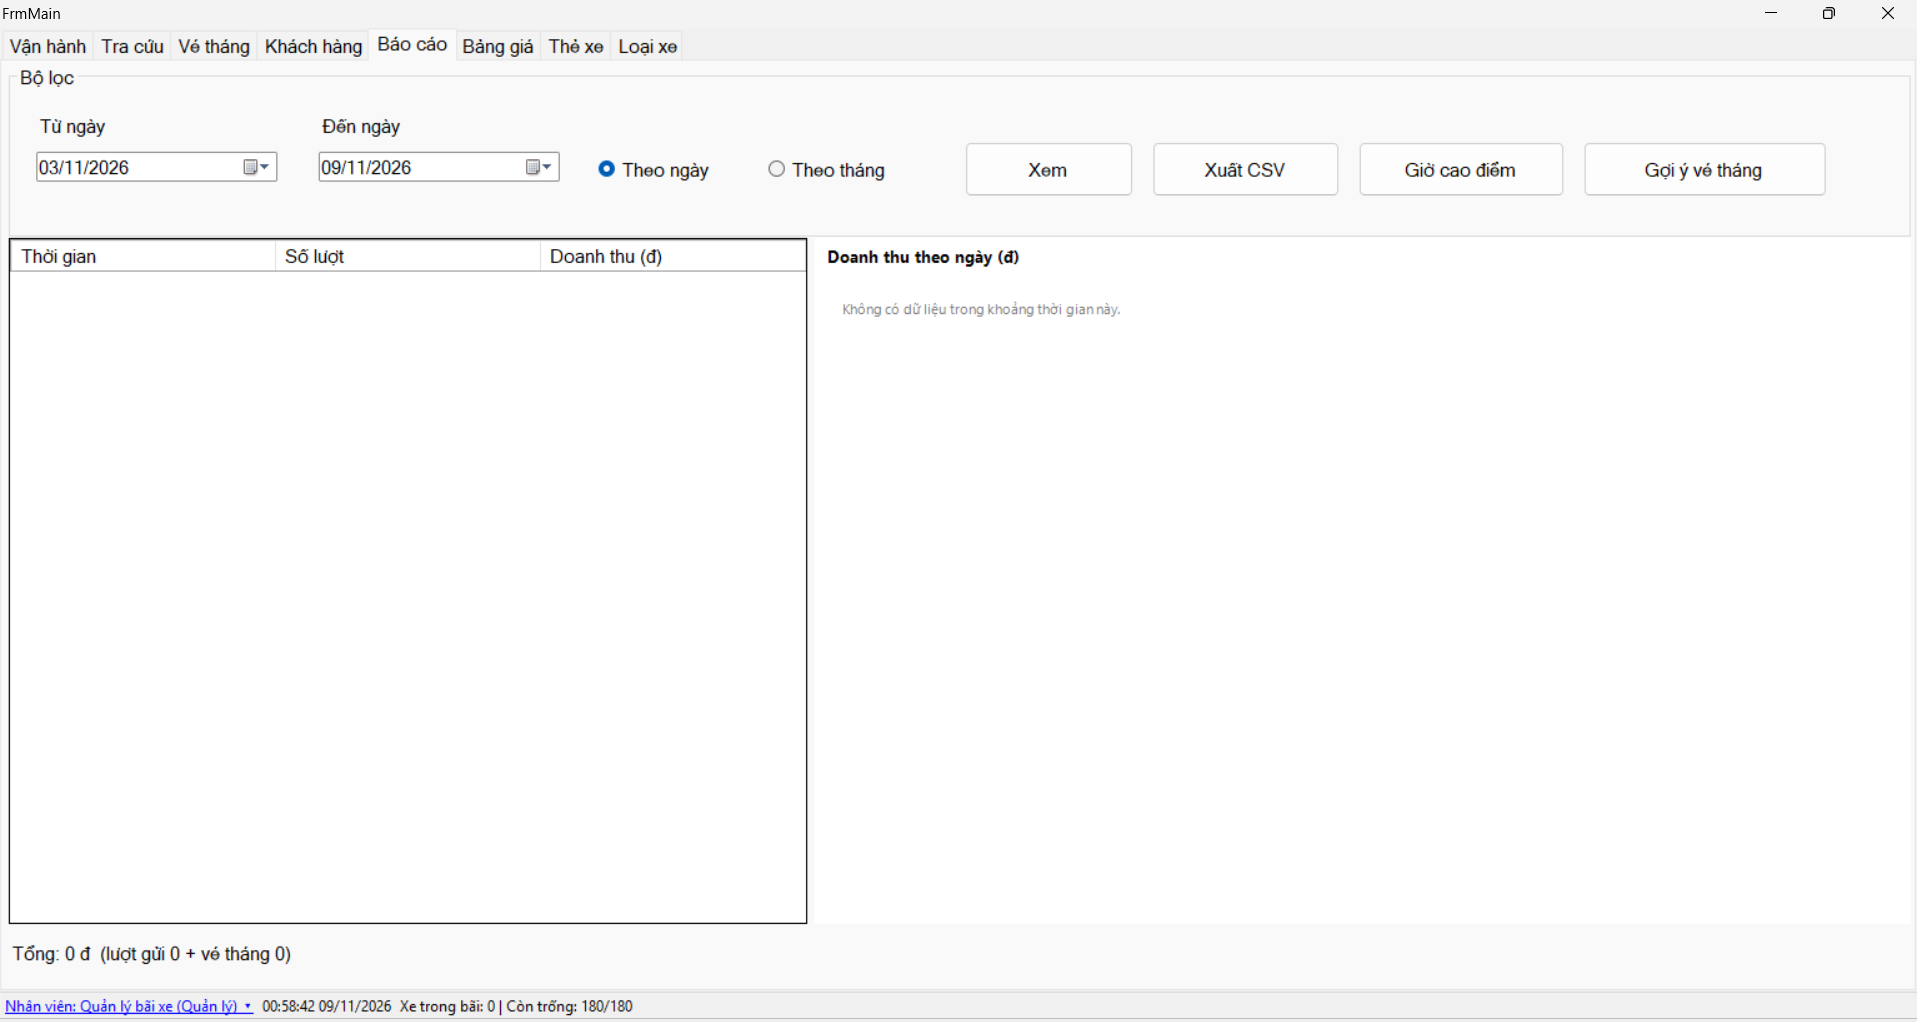
\includegraphics[width=0.6\textwidth]{images/gd-bao-cao.png}
    \caption{Giao diện thống kê doanh thu}
    \label{fig:bao-cao}
\end{figure}

% ==================================================
\section*{Kết chương}
% ==================================================

Chương này đã trình bày quá trình triển khai hệ thống quản lý bãi
giữ xe bằng C\#, WinForms và SQL Server. Các chức năng chính như
ghi nhận xe vào, xe ra, tính phí, quản lý vé tháng, tra cứu lịch
sử và in biên nhận đã được hiện thực hóa theo thiết kế ở Chương~4.

Kết quả triển khai là cơ sở để thực hiện kiểm thử và đánh giá hệ
thống trong chương tiếp theo.
```